%%%%%%%%%%%%%%%%%%%%%%%%%%%%%%%%%%%%%%%%%%%%%%%%%%%%%%%%%%%%%%%%%%%%%%%%%%%%%%%%
% Template for USENIX papers.
%
% History:
%
% - TEMPLATE for Usenix papers, specifically to meet requirements of
%   USENIX '05. originally a template for producing IEEE-format
%   articles using LaTeX. written by Matthew Ward, CS Department,
%   Worcester Polytechnic Institute. adapted by David Beazley for his
%   excellent SWIG paper in Proceedings, Tcl 96. turned into a
%   smartass generic template by De Clarke, with thanks to both the
%   above pioneers. Use at your own risk. Complaints to /dev/null.
%   Make it two column with no page numbering, default is 10 point.
%
% - Munged by Fred Douglis <douglis@research.att.com> 10/97 to
%   separate the .sty file from the LaTeX source template, so that
%   people can more easily include the .sty file into an existing
%   document. Also changed to more closely follow the style guidelines
%   as represented by the Word sample file.
%
% - Note that since 2010, USENIX does not require endnotes. If you
%   want foot of page notes, don't include the endnotes package in the
%   usepackage command, below.
% - This version uses the latex2e styles, not the very ancient 2.09
%   stuff.
%
% - Updated July 2018: Text block size changed from 6.5" to 7"
%
% - Updated Dec 2018 for ATC'19:
%
%   * Revised text to pass HotCRP's auto-formatting check, with
%     hotcrp.settings.submission_form.body_font_size=10pt, and
%     hotcrp.settings.submission_form.line_height=12pt
%
%   * Switched from \endnote-s to \footnote-s to match Usenix's policy.
%
%   * \section* => \begin{abstract} ... \end{abstract}
%
%   * Make template self-contained in terms of bibtex entires, to allow
%     this file to be compiled. (And changing refs style to 'plain'.)
%
%   * Make template self-contained in terms of figures, to
%     allow this file to be compiled. 
%
%   * Added packages for hyperref, embedding fonts, and improving
%     appearance.
%   
%   * Removed outdated text.
%
%%%%%%%%%%%%%%%%%%%%%%%%%%%%%%%%%%%%%%%%%%%%%%%%%%%%%%%%%%%%%%%%%%%%%%%%%%%%%%%%

\documentclass[letterpaper,twocolumn,10pt]{article}
\usepackage{usenix2019_v3}

% to be able to draw some self-contained figs
\usepackage{tikz}
\usetikzlibrary{arrows.meta, fit, positioning, calc}
\usepackage{amsmath}
% \usepackage{algorithm}
% \usepackage{algpseudocode}
\usepackage[ruled,linesnumbered]{algorithm2e}
% inlined bib file
\usepackage{filecontents}

%-------------------------------------------------------------------------------
\begin{filecontents}{\jobname.bib}
%-------------------------------------------------------------------------------
@Book{arpachiDusseau18:osbook,
  author =       {Arpaci-Dusseau, Remzi H. and Arpaci-Dusseau Andrea C.},
  title =        {Operating Systems: Three Easy Pieces},
  publisher =    {Arpaci-Dusseau Books, LLC},
  year =         2015,
  edition =      {1.00},
  note =         {\url{http://pages.cs.wisc.edu/~remzi/OSTEP/}}
}
@InProceedings{waldspurger02,
  author =       {Waldspurger, Carl A.},
  title =        {Memory resource management in {VMware ESX} server},
  booktitle =    {USENIX Symposium on Operating System Design and
                  Implementation (OSDI)},
  year =         2002,
  pages =        {181--194},
  note =         {\url{https://www.usenix.org/legacy/event/osdi02/tech/waldspurger/waldspurger.pdf}}}
\end{filecontents}

\newcommand{\showkot}[1]{ {\color{red}{#1}}}
% \newcommand{\ours}{\xspace MtCache \xspace}
\newcommand{\ours}{SieveDB}
%-------------------------------------------------------------------------------
\begin{document}
%-------------------------------------------------------------------------------

%don't want date printed
\date{}

% make title bold and 14 pt font (Latex default is non-bold, 16 pt)
\title{\Large \bf \ours : Pushdown and Caching in Decentralized Databases}

%for single author (just remove % characters)
% \author{
% {\rm Your N.\ Here}\\
% Your Institution
% \and
% {\rm Second Name}\\
% Second Institution
% % copy the following lines to add more authors
% % \and
% % {\rm Name}\\
% %Name Institution
% } % end author

\maketitle

%-------------------------------------------------------------------------------
\begin{abstract}
%-------------------------------------------------------------------------------
\showkot{Write later.}
\end{abstract}


%-------------------------------------------------------------------------------
\section{Introduction}
%-------------------------------------------------------------------------------
\showkot{Write later.} \\
Decentralized databases built on peer-to-peer (P2P) storage networks, such as the InterPlanetary File System (IPFS), offer resistance to censorship, data sovereignty, and fault tolerance, but come at a steep price in query performance. Every data access requires one or more P2P network fetches -- each orders of magnitude slower than a local disk read, making network I/O the dominant bottleneck~\cite{trautwein2022design, henningsen2020mapping, daniel2022ipfs}. Although decades of research have optimized cache and indexing for centralized and cloud-hosted databases~\cite{graefe2011modern, armbrust2021lakehouse}, these techniques assume low-latency local storage and do not apply to decentralized settings where queries must traverse Merkle DAGs over content-addressed P2P networks.

\section{Background and Motivation}
 
This section describes the architecture of decentralized database systems built on peer-to-peer (P2P) storage (Section~\ref{sec:bg_arch}) and the performance challenges that motivate \ours{} (Section~\ref{sec:bg_challenges}).
 
\subsection{Decentralized DBMS Architecture}
\label{sec:bg_arch}
 
Decentralized databases replace centrally administered storage with content-addressed P2P networks such as the InterPlanetary File System (IPFS)~\cite{benet2014ipfs}. In IPFS, every object is identified by a cryptographic Content Identifier (CID) derived from the object's contents. Objects are organized into Merkle DAGs~\cite{merkle1987digital} and located via a Kademlia-based distributed hash table (DHT). This architecture provides censorship resistance, data sovereignty, and fault tolerance without a single point of failure, but it fundamentally changes the data access model compared to centralized or cloud-hosted databases.
 
In a conventional cloud DBMS, data resides on local disks or cloud-attached block storage (e.g., Amazon S3), where a cache miss incurs microseconds of latency. Modern cloud-native systems adopt a \emph{storage-disaggregation} architecture that separates compute and storage into independently scalable layers~\cite{dageville2016snowflake, yang2021flexpushdowndb}. The network connecting these layers is a well-provisioned data-center fabric with bandwidth on the order of 10--50~Gbps and round-trip latencies below 1~ms.
 
A decentralized DBMS replaces this cloud storage layer with IPFS. Figure~\ref{fig:arch} illustrates three representative architectures along a spectrum of increasing optimization. In the \emph{monolithic} design (Figure~\ref{fig:arch}(a)), the query engine fetches all required data from IPFS into local memory before processing; every query pays the full P2P retrieval cost. Systems such as BigchainDB~\cite{mcconaghy2016bigchaindb} and early IPFS-backed stores follow this model.
 
In the \emph{blockchain-coordinated} design (Figure~\ref{fig:arch}(b)), an on-chain index records partition metadata and access-control policies while data remains on IPFS. MtDB~\cite{hossain2025mtdb} and Web3DB~\cite{mukherjee2025web3db} adopt this architecture: smart contracts manage table schemas and partition CIDs, and a trusted execution environment (TEE) processes queries over encrypted data. Blockchain coordination enables secure multi-tenant data sharing but does not reduce the volume of data fetched from IPFS per query.
 
The \emph{hybrid} architecture (Figure~\ref{fig:arch}(c)), which \ours{} adopts, extends the blockchain-coordinated model with two new components at the compute layer: a \emph{semantic cache} that retains query results inside the TEE, and a \emph{pushdown-aware data organization} layer that restructures table data on IPFS so that query predicates can prune irrelevant objects before retrieval. Analogous to how cloud-native systems exploit caching and computation pushdown within a disaggregated fabric~\cite{yang2021flexpushdowndb}, \ours{} introduces mechanisms to mitigate the far more severe network penalty of P2P content retrieval.

\begin{figure*}[t]
    \centering
    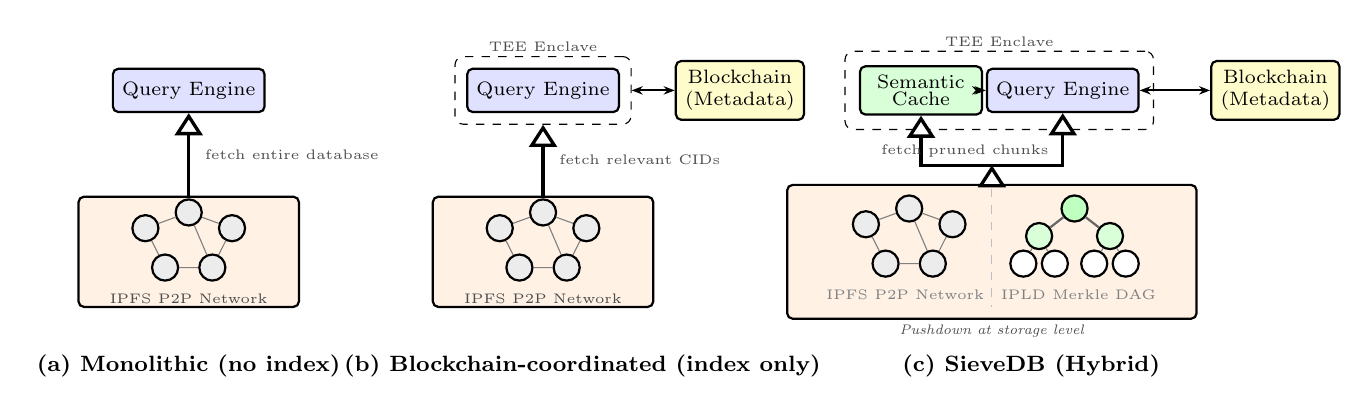
\begin{tikzpicture}[
    box/.style={draw, rounded corners=2pt, minimum width=1.7cm,
                minimum height=0.55cm, font=\scriptsize, align=center, thick},
    ipfsnode/.style={draw, circle, minimum size=0.3cm, font=\tiny,
                     thick, fill=gray!15},
    dagnode/.style={draw, circle, minimum size=0.25cm, thick, fill=white},
    hollowarrow/.style={
        -{Triangle[length=8pt, width=10pt, fill=white]},
        line width=1.2pt, draw=black
    },
    thinarrow/.style={
        -{Stealth[length=4pt]}, thick
    },
    doublearrow/.style={
        {Stealth[length=4pt]}-{Stealth[length=4pt]}, thick
    },
    labelstyle/.style={font=\footnotesize\bfseries},
    annot/.style={font=\tiny, text=black!70},
]
 
\def\ytop{0}
\def\ynet{-2.05}
\def\ylabel{-3.5}
 
%% =====================================================================
%%  (a) Monolithic
%% =====================================================================
\begin{scope}[shift={(0,0)}]
    \node[box, fill=blue!12] (qe-a) at (0,\ytop) {Query Engine};
 
    \node[box, fill=orange!10, minimum width=2.8cm,
          minimum height=1.4cm] (p2p-a) at (0,\ynet) {};
 
    \node[ipfsnode] (n1a) at (-0.55,-1.75) {};
    \node[ipfsnode] (n2a) at ( 0.0, -1.55) {};
    \node[ipfsnode] (n3a) at ( 0.55,-1.75) {};
    \node[ipfsnode] (n4a) at (-0.3, -2.25) {};
    \node[ipfsnode] (n5a) at ( 0.3, -2.25) {};
    \draw[thin, gray]
        (n1a)--(n2a) (n2a)--(n3a) (n1a)--(n4a)
        (n4a)--(n5a) (n3a)--(n5a) (n2a)--(n5a);
 
    \node[annot] at (0,-2.65) {IPFS P2P Network};
 
    \draw[hollowarrow]
        (p2p-a.north) -- node[right, annot, xshift=2pt] {fetch entire database}
        (qe-a.south);
 
    \node[labelstyle] at (0,\ylabel) {(a) Monolithic (no index)};
\end{scope}
 
%% =====================================================================
%%  (b) Blockchain-coordinated
%% =====================================================================
\begin{scope}[shift={(4.5,0)}]
    \node[box, fill=blue!12, minimum width=1.8cm] (qe-b) at (0,\ytop)
        {Query Engine};
    \node[draw, dashed, rounded corners=3pt, inner sep=4pt, fit=(qe-b),
          label={[annot, yshift=-2pt]above:TEE Enclave}] (tee-b) {};
 
    \node[box, fill=yellow!20, minimum width=1.5cm] (bc-b) at (2.5,\ytop)
        {Blockchain\\(Metadata)};
 
    \node[box, fill=orange!10, minimum width=2.8cm,
          minimum height=1.4cm] (p2p-b) at (0,\ynet) {};
 
    \node[ipfsnode] (n1b) at (-0.55,-1.75) {};
    \node[ipfsnode] (n2b) at ( 0.0, -1.55) {};
    \node[ipfsnode] (n3b) at ( 0.55,-1.75) {};
    \node[ipfsnode] (n4b) at (-0.3, -2.25) {};
    \node[ipfsnode] (n5b) at ( 0.3, -2.25) {};
    \draw[thin, gray]
        (n1b)--(n2b) (n2b)--(n3b) (n1b)--(n4b)
        (n4b)--(n5b) (n3b)--(n5b) (n2b)--(n5b);
 
    \node[annot] at (0,-2.65) {IPFS P2P Network};
 
    \draw[hollowarrow]
        (p2p-b.north) -- node[right, annot, xshift=2pt] {fetch relevant CIDs}
        (tee-b.south);
 
    \draw[doublearrow] (tee-b.east) -- (bc-b.west);
 
    \node[labelstyle] at (0.5,\ylabel)
        {(b) Blockchain-coordinated (index only)};
\end{scope}
 
%% =====================================================================
%%  (c) Hybrid (SieveDB)
%% =====================================================================
\begin{scope}[shift={(10.2,0)}]
    %% Cache and QE side-by-side
    \node[box, fill=green!15, minimum width=1.55cm] (cache-c) at (-0.9, \ytop)
        {Semantic\\[-2pt]Cache};
    \node[box, fill=blue!12,  minimum width=1.55cm] (qe-c)    at ( 0.9, \ytop)
        {Query Engine};
 
    \draw[doublearrow]
        (cache-c.east) -- (qe-c.west);
 
    \node[draw, dashed, rounded corners=3pt, inner sep=5pt,
          fit=(cache-c)(qe-c),
          label={[annot, yshift=-2pt]above:TEE Enclave}] (tee-c) {};
 
    \node[box, fill=yellow!20, minimum width=1.5cm] (bc-c) at (3.6, \ytop)
        {Blockchain\\(Metadata)};
    \draw[doublearrow] (qe-c.east) -- (bc-c.west);
 
    %% IPFS + Merkle DAG storage box
    \node[box, fill=orange!10, minimum width=5.2cm,
          minimum height=1.7cm] (p2p-c) at (0, \ynet) {};
 
    %% Left half: P2P network nodes
    \node[ipfsnode] (n1c) at (-1.6,-1.7) {};
    \node[ipfsnode] (n2c) at (-1.05,-1.5) {};
    \node[ipfsnode] (n3c) at (-0.5,-1.7) {};
    \node[ipfsnode] (n4c) at (-1.35,-2.2) {};
    \node[ipfsnode] (n5c) at (-0.75,-2.2) {};
    \draw[thin, gray]
        (n1c)--(n2c) (n2c)--(n3c) (n1c)--(n4c)
        (n4c)--(n5c) (n3c)--(n5c) (n2c)--(n5c);
 
    %% Divider line
    \draw[thin, gray!50, dashed] (0, -1.25) -- (0, -2.75);
 
    %% Right half: Merkle DAG tree
    \node[dagnode, fill=green!25] (dag-root) at (1.05, -1.5) {};
    \node[dagnode, fill=green!15] (dag-l1) at (0.6, -1.85) {};
    \node[dagnode, fill=green!15] (dag-r1) at (1.5, -1.85) {};
    \node[dagnode] (dag-l2a) at (0.4, -2.2) {};
    \node[dagnode] (dag-l2b) at (0.8, -2.2) {};
    \node[dagnode] (dag-r2a) at (1.3, -2.2) {};
    \node[dagnode] (dag-r2b) at (1.7, -2.2) {};
    \draw[thick, black!60] (dag-root) -- (dag-l1);
    \draw[thick, black!60] (dag-root) -- (dag-r1);
    \draw[thin,  black!50] (dag-l1) -- (dag-l2a);
    \draw[thin,  black!50] (dag-l1) -- (dag-l2b);
    \draw[thin,  black!50] (dag-r1) -- (dag-r2a);
    \draw[thin,  black!50] (dag-r1) -- (dag-r2b);
 
    %% Sub-labels inside IPFS box
    \node[font=\tiny, text=black!50] at (-1.1, -2.6) {IPFS P2P Network};
    \node[font=\tiny, text=black!50] at (1.1, -2.6)  {IPLD Merkle DAG};
 
    %% Annotation below storage box
    \node[annot, font=\tiny\itshape] at (0,-3.05) {Pushdown at storage level};
 
    %% Fork: IPFS splits to cache and QE
    \coordinate (fork) at (0,-0.95);
 
    %% Stem from IPFS to fork
    \draw[hollowarrow] (p2p-c.north) -- (fork);
 
    %% Left branch -> cache
    \draw[hollowarrow]
        (fork) -- (-0.9,-.95) -- node[left, annot, xshift=50pt, yshift=-4pt] {fetch pruned chunks} (cache-c.south);
 
    %% Right branch -> QE
    \draw[hollowarrow]
        (fork) -- (0.9,-0.95) -- (qe-c.south);
 
    \node[labelstyle] at (0.5,\ylabel) {(c) \ours{} (Hybrid)};
\end{scope}
 
\end{tikzpicture}
    \caption{Decentralized database architectures -- (a)~monolithic: the query engine fetches all data from IPFS; (b)~blockchain-coordinated: a TEE-based engine uses on-chain metadata but still fetches all relevant data; (c)~hybrid (\ours{}): a semantic cache and pushdown DAG reduce IPFS fetches.}
    \label{fig:arch}
\end{figure*}
 
\subsection{Challenges in Decentralized DBMSs}
\label{sec:bg_challenges}
 
The P2P network connecting the query engine to IPFS storage is the dominant performance bottleneck in decentralized databases. Unlike cloud data-center networks, where bandwidth is abundant and latency is sub-millisecond, IPFS retrieval involves multi-hop DHT lookups, content routing, and data transfer across the Wide Area Network (WAN). Large-scale measurements report median retrieval latencies of 2--5~seconds for unpinned content, with individual DHT hops adding hundreds of milliseconds~\cite{trautwein2022design, henningsen2020mapping, daniel2022ipfs}. Even pinned content on well-connected peers exhibits round-trip latencies one to two orders of magnitude higher than cloud-attached storage, making a single table scan over IPFS 100--1000$\times$ slower than the equivalent scan over S3 or local SSD.
 
Two complementary techniques have been explored in cloud databases to mitigate a similar (though far less severe) bottleneck between compute and storage layers: \emph{caching} and \emph{computation pushdown}~\cite{yang2021flexpushdowndb}. We examine how each translates to the decentralized setting and why neither alone is sufficient.
 
\paragraph{Caching.}
Caching keeps recently accessed data in the compute node's local memory or on attached SSD, eliminating P2P network fetches for repeated accesses. In cloud databases, a cache miss is inexpensive---a few milliseconds to fetch from S3. In a decentralized DBMS, the miss penalty is 100--5000$\times$ higher, making each cache hit proportionally more valuable but each poor eviction decision far more costly. The cache resides inside a TEE enclave with limited memory (e.g., 128~GB under SGX~v2~\cite{costan2016intel}) \showkot{verify enclave memory size}, so the eviction policy must carefully prioritize entries by their expected future value.
 
Existing cloud caching systems~\cite{dageville2016snowflake, melnik2010dremel, fitzpatrick2004distributed} key cache entries by exact query strings or buffer-pool page identifiers. These approaches cannot exploit overlap between queries: a cached result for \texttt{Age > 50} is invisible to a subsequent query for \texttt{Age > 60}, even though the latter is fully contained in the former. In the decentralized setting, where each miss is catastrophically expensive, exploiting such semantic overlap is critical.
 
\paragraph{Computation pushdown.}
Computation pushdown moves filtering and aggregation closer to the storage layer, reducing the volume of data transferred over the network. Cloud systems such as S3 Select and Redshift Spectrum~\cite{yang2021flexpushdowndb} support native filter evaluation at the storage service, but IPFS provides no analogous query interface---it is a content-addressed object store with no awareness of relational schemas or predicates. Requesting an object by its CID returns the entire object; there is no mechanism to retrieve a filtered subset.
 
Enabling pushdown in a decentralized DBMS, therefore, requires \emph{reorganizing the data on IPFS} so that the IPFS node can determine which chunks are relevant to a given predicate. This is fundamentally different from cloud pushdown, where the storage service itself evaluates the predicates. In the decentralized setting, we need to create semantic-aware data partitions and a custom Merkle DAG to support pushdown at the storage (IPFS) level. We will describe this in section \ref{}.
 
\paragraph{The case for a hybrid approach.}
Existing decentralized database systems support neither caching nor pushdown, leaving the full P2P retrieval cost on the critical path of every query~\cite{hossain2025mtdb, mukherjee2025web3db, yao2024minerva}. Moreover, the two techniques are not orthogonal: a system that only caches must still fetch every cold-miss object in full, while a system that only pushes down predicates gains nothing from repeated queries over the same data. The extreme cost asymmetry in decentralized storage---where a cache hit costs microseconds and a miss costs seconds---amplifies the benefit of combining both approaches.
 
\ours{} addresses this gap with a hybrid design. Its semantic cache reuses cached results across queries via SMT-based predicate containment, and its pushdown layer organizes table data into a metadata-rich IPLD Merkle DAG that enables predicate-based pruning at the IPFS level. Together, these mechanisms reduce P2P fetches from both directions: the cache eliminates fetches for overlapping queries, while the pushdown DAG eliminates fetches for irrelevant data partitions.

\section{\ours{} Overview}

\subsection{System Architecture}
\textbf{Block reorganizer.} \\
\textbf{Cache manager.} \\
\textbf{Hybrid query engine.}
\subsection{Desing Choices}
\textbf{Caching of Table Data or Query Results.} \\
\textbf{Partitioning and Caching Granularity.}

\section{Hybrid Query Engine}
\subsection{Separable Operators}
\subsection{Separable Query Plan}
\subsection{Example Query Execution}

\section{Cache Manager}
\subsection{Integration with Hybrid Query Engine}
\subsection{Utility-Aware Caching Framework}
\subsection{Traditional Cache Eviction Policy}
\subsection{Semantic Sieve Eviction Policy}

\section{Implementation}
\subsection{Decentralized Storage}
\subsection{Data Format}
\subsection{In-Enclave Parallel Processing}

\section{Evaluation}


\section{Related Work}
\label{sec:litreview}
\showkot{Need to shorten later.}
% This review surveys work that informs \ours{}, which contributes (1)~a TEE-based, multi-layer semantic-aware caching system with SMT-based query containment, and (2)~a content-addressed, multi-dimensional sharding technique that enables predicate pushdown at the IPFS storage layer.

%% ---------------------------------------------------------------
\subsection{IPFS and Decentralized Databases}
\label{sec:ipfs}
%% ---------------------------------------------------------------

IPFS~\cite{benet2014ipfs} introduced content-addressed storage on a Kademlia-based DHT with Merkle DAG data structures, where every object is identified by its cryptographic Content Identifier (CID). Large-scale measurements report that the median IPFS retrieval latency is 2-5 seconds for unpinned content, with multi-hop DHT lookups adding hundreds of milliseconds per round~\cite{trautwein2022design, henningsen2020mapping, daniel2022ipfs}. While IPLD~\cite{ipld2023spec} provides a linked-data model layer atop IPFS, it doesn't natively support pushdown storage-level filtering for relational data to reduce I/O costs.

Several systems build database abstractions on decentralized storage. Early efforts, such as BigChainDB~\cite{mcconaghy2016bigchaindb}, overlay database semantics on blockchain consensus but inherit throughput limitations, while key-value and document interfaces on IPFS lack relational query support. Minerva~\cite{yao2024minerva} distributes query execution across IPFS peers with a cost-based planner but does not incorporate caching or predicate-aware data organization, leaving content retrieval latency unaddressed.

Most relevant to our work are MtDB~\cite{hossain2025mtdb} and Web3DB~\cite{mukherjee2025web3db}. MtDB integrates IPFS storage, Ethereum smart contracts for metadata coordination, and Intel SGX for secure query execution; its delta-based on-chain index enables partition discovery but not predicate pushdown within a partition. Web3DB provides blockchain-managed access control for relational queries, but lacks enclave-based secure query execution. Both of these systems lack a caching or data organization layer to reduce I/O bottlenecks. \ours{} builds on MtDB's architecture, adding semantic caching and content-addressed sharding to reduce IPFS I/O and query latency.


%% ---------------------------------------------------------------
\subsection{Database Caching and Semantic Caching}
\label{sec:caching}
%% ---------------------------------------------------------------

Traditional database caching -- buffer pools~\cite{graefe2011modern}, key-value stores such as Memcached~\cite{fitzpatrick2004distributed}, Redis~\cite{redis2009} and result caches in cloud warehouses~\cite{dageville2016snowflake, melnik2010dremel} -- reduces I/O to local or cloud-attached disk, where cache miss penalties are microseconds. In distributed settings, DistCache~\cite{liu2019distcache} provides provably balanced caching for large-scale storage, Crystal~\cite{durner2021crystal} unifies columnar and row-based caching for analytics, and the work of Tang et al.~\cite{tang2024data} coordinates multi-layer caching for petabyte-scale OLAP. Metadata caching in Presto~\cite{wang2022metadata} eliminates redundant metastore calls, while HyCache~\cite{zhao2013hycache} interposes application-aware caching in distributed file systems. All these systems target predictable, low-latency storage and do not address the fundamentally different cost model of P2P content retrieval, where a cache miss costs 100-5000 ms.

Result caches keyed by normalized SQL strings~\cite{dageville2016snowflake, melnik2010dremel} cannot exploit overlap between queries: a query for \texttt{Age > 60} is a miss even if \texttt{Age > 50} is cached. Semantic caching addresses this by annotating cached results with defining predicates and checking containment~\cite{dar1996semantic}. Keller and Basu~\cite{keller1996predicate} extended the approach with predicate indices, and Roy et al.~\cite{roy2000don} advocated caching intermediate results for cross-query reuse. Most recently, You et al. \cite{you2025soc} propose succinct semantic representations for OLAP caching but rely on heuristic predicate overlap rather than formal containment, and target cloud warehouses with fast storage. We use SMT-based containment via Z3~\cite{de2008z3} to guarantee soundness, and the extreme IPFS miss penalty makes the 2-15 ms predicate-checking overhead negligible.

Cache eviction is a core component of any caching system -- especially in an in-memory cache, given limited storage capacity. For eviction, classical policies \cite{megiddo2003arc, einziger2017tinylfu,jiang2002lirs,zhang2024sieve} treat each cache object as opaque. Recently, the SIEVE algorithm~\cite{zhang2024sieve} achieves both eager promotion and quick demotion of cache entries using a single visited bit, but it ignores semantic relationships, which are essential in our scenario. Cost-aware eviction consistently outperforms cost-oblivious policies~\cite{podlipnig2003survey} when cache miss cost is high (e.g., 100--5000 ms). Our cache eviction algorithm augments SIEVE with a second utility bit encoding the semantic reuse potential of each entry, preserving O(1) complexity.


%% ---------------------------------------------------------------
\subsection{Query Containment and Predicate Pushdown}
\label{sec:containment}
%% ---------------------------------------------------------------

Query containment -- determining whether one query's results are a subset of another's -- was formalized by Chandra and Merlin~\cite{chandra1977optimal} as NP-complete for conjunctive queries. SMT solvers~\cite{de2008z3} provide a natural encoding for containment checks. VeriEQL~\cite{he2024verieql} leverages Z3 for bounded equivalence verification of SQL queries under integrity constraints, while Cosette~\cite{chu2017cosette} approaches query equivalence via symbolic constraint solving. These systems are designed for offline verification; in contrast, our containment checker operates online, where soundness (no false positives) is required but incompleteness is acceptable.

Predicate pushdown is a standard optimization in lakehouse and columnar systems~\cite{armbrust2021lakehouse}. FlexPushdownDB~\cite{yang2021flexpushdowndb} dynamically decides whether to push predicates to cloud storage (e.g., S3 Select) or process them locally, trading off network cost against computation. In decentralized databases~\cite{hossain2025mtdb, mukherjee2025web3db}, however, the pushdown target is not a cloud service with native filtering support, but an IPFS node that exposes no query interface. We address this gap by constructing a custom DAG over IPFS that encodes range metadata using IPLD~\cite{ipld2023spec}, enabling predicate filtering at the storage layer without any intermediate middleware. To our knowledge, no prior work has achieved pushdown filtering directly at the IPFS level.


%% ---------------------------------------------------------------
\subsection{Data Sharding and Indexing}
\label{sec:sharding}
%% ---------------------------------------------------------------

Range, hash, and composite partitioning are well-established for parallel databases~\cite{dewitt1992parallel}. Cloud-native systems like CockroachDB~\cite{taft2020cockroachdb} and Spanner~\cite{bacon2017spanner} use adaptive range partitioning with automatic shard splitting. DynaHash~\cite{luo2022dynahash} addresses efficient data rebalancing in AsterixDB via extensible hashing. All assume mutable, low-latency storage; IPFS's immutable content-addressed model requires constructing new Merkle DAGs rather than rebalancing in place.

Indexing for decentralized storage remains limited. Existing IPFS indexing frameworks target key-value or keyword lookups~\cite{arer2022efficient}, and blockchain-anchored indices focus on provenance~\cite{rathee2019blockchain} rather than query optimization. The Merkle DAG~\cite{benet2014ipfs, merkle1987digital} is a natural index for content-addressed systems. Our technique constructs a custom DAG in which internal nodes record min/max ranges across multiple attributes, enabling top-down traversal with branch pruning -- analogous to B$^+$-tree scans but adapted to immutable IPFS. Learned indices~\cite{kraska2018case} and related adaptive indexing techniques assume mutable storage and do not transfer to our setting.


%% ---------------------------------------------------------------
\subsection{TEE and Blockchain-based Databases}
\label{sec:tee}
%% ---------------------------------------------------------------

Trusted execution environments (TEEs) provide isolated execution with protected memory and confidentiality guarantees. Intel SGX~\cite{costan2016intel}, one of the most widely used TEEs, supports application-level enclaves and remote attestation. TEEs are well-suited for secure database caching, where both the cache state and the query execution logic can be carefully scoped to fit within enclave memory.

Several database systems have leveraged TEEs for secure query processing. EnclaveDB~\cite{priebe2018enclavedb} executes SQL operators inside SGX enclaves, while Opaque~\cite{zheng2017opaque} integrates SGX with Spark to support secure data analytics. CryptDB~\cite{popa2011cryptdb}, although not TEE-based, enables SQL queries over encrypted data using adjustable encryption schemes, but still leaks access patterns. However, these systems are designed for local or cloud-backed storage environments with relatively low-latency data access. As a result, they do not address the core challenges of peer-to-peer storage latency.

A related line of work combines blockchain systems with confidential computation. For example, Enigma~\cite{zyskind2018enigma} uses blockchain coordination together with privacy-preserving computation, but its primary goal is computation confidentiality rather than query acceleration. Similarly, verifiable query processing systems such as vChain~\cite{xu2019vchain} focus on correctness guarantees through cryptographic proofs, often incurring additional overhead without improving latency. MtDB~\cite{hossain2025mtdb} provides the underlying blockchain-based metadata coordination model that we build upon. In contrast, \ours{} introduces new mechanisms entirely at the off-chain caching and data-organization layers, targeting lower query latency and higher efficiency for decentralized database workloads.

\section{Methodology}

\subsection{Pushdown: Content-Addressed Multidimensional Sharding}

\ours{} reduces the latency of decentralized databases by taking two key steps in the data organization layer. First, it partitions each table into content-addressed shards whose sizes match the granularity at which IPFS efficiently transports data. Second, it organizes those shards into a metadata-rich IPLD\cite{ipld2023spec} Merkle DAG, allowing query predicates to prune irrelevant subtrees before any shard is fetched. Together, these mechanisms enable predicate pushdown over a relational table stored in IPFS.

The dominant cost in IPFS-backed query processing is not local scan time, but the number and the size of remote object retrievals. In practice, fetching a single block incurs a network round-trip; fetching many blocks multiplies that cost. Our sharding strategy, therefore, targets two properties: (1) each shard should be close to the IPFS default transfer unit to avoid underfilled/fragmented objects, and (2) shards should be organized so that predicates can exclude large portions of the table without retrieving them.

\subsubsection{Extended KD-Tree Partitioning}
\label{sec:partitioning}

Given a table $T$ with $N$ rows and a set of partitioning attributes $A = \{a_1, \ldots, a_d\}$, we construct shards $\{S_1, \ldots, S_k\}$ such that:

\begin{itemize}
    \item each shard $S_i$ corresponds to a contiguous, range-bounded region in the $d$-dimensional attribute space;
    \item the serialized size of each shard is close to a target size $\tau$ (default 256\,KB, matching the IPFS block size);
    \item each shard stores a bounding box $\mathcal{B}(S_i) = \{(a_j, [\min_j, \max_j])\}_{j=1}^{d}$ that summarizes its value ranges.
\end{itemize}

We generate these shards with a recursive, size-aware variant of a KD-tree. At each recursion step, the algorithm chooses the split attribute whose values span the widest \emph{normalized} range within the current subset:
\begin{equation}
    a^* = \arg\max_{a_j \in A} \; \frac{\max(a_j) - \min(a_j)}{R_j^{\text{global}}}
    \label{eq:split_attr}
\end{equation}
where $R_j^{\text{global}} = \max_T(a_j) - \min_T(a_j)$ is the global range of attribute $a_j$ in the full table. This normalization prevents high-magnitude attributes from dominating the split decision purely because of scale. For example, it allows attributes such as \texttt{Age} and \texttt{Salary} to be compared fairly even though their numeric domains differ substantially.

After selecting $a^*$, we split the current subset at the median value of that attribute. Median splitting keeps the tree balanced, while the adaptive choice of split dimension keeps shards spatially tight in the attributes most useful for pruning. To control shard size, we estimate the average compressed Parquet size per row as $\hat{r}$ and derive the target number of rows per shard as $n_{\text{target}} = \lfloor \tau / \hat{r} \rfloor$. Recursion stops when a subset contains at most $n_{\text{target}}$ rows, or when further splitting would create an empty child.

\begin{algorithm}[t]
\caption{\textsc{Extended-KD-Partition} for multidimensional sharding}
\label{alg:partition}
\DontPrintSemicolon
\KwIn{Table $T$ with $N$ rows, attributes $A = \{a_1, \ldots, a_d\}$, target shard size $\tau$}
\KwOut{Shards $\{S_1, \ldots, S_k\}$}
$\hat{r} \gets \text{EstimateRowSize}(T)$\;
$n_{\text{target}} \gets \lfloor \tau / \hat{r} \rfloor$\;
$R^{\text{global}} \gets \{(a_j, \max_T(a_j) - \min_T(a_j))\}_{j=1}^{d}$\;
\Return \textsc{Recurse}($T$, $A$, $R^{\text{global}}$, $n_{\text{target}}$, depth=0)\;
\BlankLine
\SetKwFunction{FRecurse}{Recurse}
\SetKwProg{Fn}{Function}{:}{}
\Fn{\FRecurse{$D$, $A$, $R^{\text{global}}$, $n_{\text{target}}$, depth}}{
    \If{$|D| \leq n_{\text{target}}$}{
        \Return $\{\text{MakeShard}(D)\}$\;
    }
    $a^* \gets \arg\max_{a_j} \frac{\max_D(a_j) - \min_D(a_j)}{R_j^{\text{global}}}$\;
    $v_{\text{med}} \gets \text{median}(D[a^*])$\;
    $D_L \gets \{r \in D : r[a^*] \leq v_{\text{med}}\}$\;
    $D_R \gets \{r \in D : r[a^*] > v_{\text{med}}\}$\;
    \If{$D_L = \emptyset$ \textbf{or} $D_R = \emptyset$}{
        \Return $\{\text{MakeShard}(D)\}$
    }
    \Return \FRecurse{$D_L$, $A$, $R^{\text{global}}$, $n_{\text{target}}$, depth$+1$} $\cup$ \FRecurse{$D_R$, $A$, $R^{\text{global}}$, $n_{\text{target}}$, depth$+1$}\;
}
\end{algorithm}

This partitioning step produces shards that are both network-efficient and semantically meaningful: each shard is small enough to retrieve efficiently from IPFS, and its bounding box can later be used for predicate-based pruning.

\subsubsection{IPLD Merkle DAG Construction}
\label{sec:dag_construction}

As described in \ref{sec:partitioning}, partitioning only reduces the size of the shards, but does not tell the system which shards to fetch for a given query. To support predicate pushdown, \ours{} builds a custom Merkle DAG over the shards using IPLD\cite{ipld2023spec}, the linked-data layer of IPFS. The key idea is to attach range metadata to internal DAG nodes so that query predicates can be evaluated during traversal. Unlike the default IPFS Merkle DAG, which is organized around byte-level chunking and is oblivious to table semantics, our DAG is organized around relational shards and their attribute ranges.
\paragraph{Leaf nodes.}
For each shard $S_i$, the system serializes the shard to Parquet and compresses it with Snappy, which reduces storage size with low decompression overhead. It then encrypts the result with the enclave key and uploads the encrypted object to IPFS, producing a data CID $c_i^{\text{data}}$. It then creates a leaf DAG node containing: (1) an IPLD link to $c_i^{\text{data}}$, (2) the shard bounding box $\mathcal{B}(S_i)$, (3) the number of rows in the shard, and (4) the serialized size. The leaf node is stored with \texttt{dag/put} using the \texttt{dag-cbor} codec, yielding a leaf CID $c_i^{\text{leaf}}$.
\paragraph{Internal nodes.}
Leaf CIDs are grouped into batches of size $b$, where $b$ is the DAG branching factor (default $b = 4$). For each group, \ours{} constructs an internal node containing links to the child nodes and an aggregate range summary. The range summary is computed attribute-wise by taking the minimum of child lower bounds and the maximum of child upper bounds. Each internal node, therefore, summarizes the full predicate-relevant extent of its subtree.
\paragraph{Recursive aggregation.}
The system repeats this aggregation step bottom-up until only a single root node remains. The resulting root CID $c_{\text{root}}$ is recorded on the global index \showkot{(explain global index)} and serves as the entry point for subsequent query execution.

\begin{algorithm}[t]
\caption{\textsc{BuildDAG}: IPLD Merkle DAG construction}
\label{alg:dag_build}
\DontPrintSemicolon
\KwIn{Shards $\{S_1, \ldots, S_k\}$, branching factor $b$, enclave key $\kappa$}
\KwOut{Root CID $c_{\text{root}}$}
$\textit{cids} \gets []$\;
\ForEach(\tcp*[f]{parallelized}){$S_i \in \{S_1, \ldots, S_k\}$}{
    $\textit{enc} \gets \text{Encrypt}(\text{Parquet}(S_i), \kappa)$\;
    $c_i^{\text{data}} \gets \text{IPFS.add}(\textit{enc})$\;
    $\textit{leaf} \gets \{\texttt{data}: \{``\!/\!": c_i^{\text{data}}\}, \texttt{ranges}: \mathcal{B}(S_i), \texttt{rows}: |S_i| \}$\;
    $c_i^{\text{leaf}} \gets \text{IPFS.dag\_put}(\textit{leaf}, \texttt{dag\text{-}cbor})$\;
    $\textit{cids}.\text{append}(c_i^{\text{leaf}})$\;
}
\While{$|\textit{cids}| > 1$}{
    $\textit{next} \gets []$\;
    \ForEach{group $G$ of $b$ consecutive CIDs in \textit{cids}}{
        $\textit{ranges} \gets \bigcup_{c \in G} \text{FetchRanges}(c)$\;
        $\textit{node} \gets \{\texttt{children}: [\{``\!/\!": c\} \mid c \in G], \texttt{ranges}: \textit{ranges}\}$\;
        $c^{\text{int}} \gets \text{IPFS.dag\_put}(\textit{node}, \texttt{dag\text{-}cbor})$\;
        $\textit{next}.\text{append}(c^{\text{int}})$\;
    }
    $\textit{cids} \gets \textit{next}$\;
}
\Return $\textit{cids}[0]$\;
\end{algorithm}

This structure enables top-down pruning during query execution. Given a predicate, the system begins at the root and checks whether the predicate overlaps each child node's summarized range. Subtrees whose ranges cannot satisfy the predicate are discarded immediately, without retrieving any descendant shards. Only leaves whose bounding boxes intersect the predicate are fetched and decrypted by the enclave (query engine). Crucially, our custom DAG turns IPFS from a content-addressed semantically blind object store into a predicate-aware access path for relational data.

The height of the DAG is $h = \lceil \log_b k \rceil$ for $k$ shards. With the default branching factor $b = 4$ and 256\,KB shards, a 1\,GB table produces approximately 4{,}000 shards and a DAG of height $\lceil \log_4 4000 \rceil = 6$ \showkot{(Change it after experiement.)}. Because each internal node is a small CBOR-encoded metadata object (typically less than 1\,KB), the storage overhead of the index is negligible relative to the underlying data.

\subsection{Caching: Semantic-Aware Cache}

\ours{} complements pushdown with a two-tier semantic cache deployed in enclave memory and on SSD. The cache operates on two principles: (1) reuse cached results across queries via SMT-based predicate containment checking, and (2) retain high-utility entries using an extended eviction algorithm. Together, these mechanisms reduce IPFS fetches by serving future queries from cached results when their predicates are satisfied.

\subsubsection{Multi-Layer Cache Architecture}

The cache operates in two tiers:

\begin{itemize}
    \item \textbf{Tier 1 (Enclave memory):} A fast, in-memory cache for recent query results, living within the SGX enclave to preserve confidentiality. Enclave memory is limited (default 128\,GB under SGX v2), so the tier is sized to hold the most valuable results as determined by utility scoring.
    \item \textbf{Tier 2 (SSD):} A secondary cache on encrypted persistent SSD. Results that fall out of enclave memory can be sealed and stored here, remaining available for future containment checks after a decrypt-on-hit penalty.
\end{itemize}

Query execution first checks the in-memory cache. On a miss, it checks the SSD tier via deserialization. A miss from both tiers triggers an IPFS fetch via the pushdown DAG.

\subsubsection{Query Containment and Result Reuse}

When a new query arrives, \ours{} checks whether its results can be derived from a cached result via predicate containment. The key insight is that if a cached query $Q_c$ has looser (weaker) predicates than a new query $Q_n$, then $\text{result}(Q_n) \subseteq \text{result}(Q_c)$, and the cached result can serve the new query after applying additional filtering.

For example, if the cache holds a result for \texttt{SELECT * WHERE Age > 50}, and a new query \texttt{SELECT * WHERE Age > 60} arrives, the new result is a subset of the cached result. The system can filter the cached result with the additional predicate \texttt{Age > 60} instead of re-fetching from IPFS.

\ours{} uses the Z3 SMT solver~\cite{de2008z3} to check predicate containment soundly. Given a cached query $Q_c$ and new query $Q_n$, the containment checker:

\begin{enumerate}
    \item Verifies that both queries target the same table(s) and have compatible join structures (e.g., both are INNER JOIN, preserving NULL semantics).
    \item For each table, constructs a Z3 formula encoding the predicates: $P_c \wedge \neg P_n$, where $P_c$ and $P_n$ are the predicate formulas of the cached and new queries, respectively.
    \item Queries Z3: does there exist a tuple satisfying $P_n$ but not $P_c$? If the answer is SAT (satisfiable), containment fails. If UNSAT, the new query $Q_n$ is proven contained in $Q_c$.
    \item If contained, \ours{} executes $Q_n$ by filtering the cached result in-enclave using the additional predicates (\texttt{AND}'d together), avoiding IPFS entirely.
\end{enumerate}

Soundness is formally guaranteed by Z3's SMT proving: an UNSAT response proves that no counter-example exists. For JOIN queries, \ours{} enforces join type compatibility (e.g., a LEFT JOIN result cannot serve an INNER JOIN, since LEFT JOIN introduces NULL rows that are absent in INNER JOIN) to preserve semantics.

The SMT check typically requires 2--15\,ms per query, but this overhead is negligible compared to IPFS latencies of 100--5000\,ms. As a result, \ours{} favors recall over precision, checking every in-memory cache entry.

\subsubsection{Utility-Aware Eviction: Semantic Sieve}

Enclave memory is a scarce resource. \ours{} uses a utility-aware extension of the SIEVE cache eviction algorithm~\cite{zhang2024sieve} to decide which cached results to retain. SIEVE uses a single visited bit; we extend it to a 2-bit model: the Visited (V) bit tracks temporal recency, while a Utility (U) bit tracks semantic value.

Each cached result is assigned a \emph{Utility Score} at insertion time:
\begin{equation}
    U(Q) = \frac{\text{Cost}(Q)}{\text{Size}(Q)} \times \text{Retain}(Q) \times \text{Breadth}(Q)
    \label{eq:utility}
\end{equation}

where:
\begin{itemize}
    \item \textbf{Cost} is the IPFS latency incurred to fetch the source data (100--5000\,ms).
    \item \textbf{Size} is the result's memory footprint in bytes.
    \item \textbf{Retain} is 1.0 for \texttt{SELECT *} (full information), lower for projections (0.6--0.9), and 0.05 for lossy aggregations (e.g., \texttt{COUNT}).
    \item \textbf{Breadth} encodes the containment potential based on predicate types: open ranges like \texttt{Age > 50} score 0.9, while equality predicates score 0.1.
\end{itemize}

During eviction, the algorithm traverses a FIFO queue with a hand pointer and applies utility-aware rules:

\begin{itemize}
    \item \textbf{V=0, U=0} (no recent hits, low utility): Evict immediately.
    \item \textbf{V=0, U=1} (high utility, no recent hits): Check if the entry is \emph{subsumed} by another cached entry (i.e., its result can be derived from another cached result via containment). If subsumed, evict. Otherwise, decay U to 0, allowing it one more pass through the queue.
    \item \textbf{V=1} (recent hit): Reset V to 0 and skip. The entry survives this eviction pass.
\end{itemize}

This design preserves SIEVE's O(1) complexity and lockless hit path while incorporating semantic awareness. A high-utility entry (U=1) survives at most 2 cold passes before eviction, ensuring bounded memory overhead.

\subsubsection{Integration with Pushdown}

Caching and pushdown work in tandem to minimize IPFS I/O. A new query is first checked against the cache via containment. If a hit is found, any additional filter predicates are applied in-enclave to produce the final result. If no cache hit, the query traverses the pushdown DAG to identify relevant IPFS shards, fetches them, decrypts them within the enclave, and inserts the result into the cache for potential reuse by future queries.

The multi-tier cache thus reduces IPFS I/O on two fronts: (1) by serving overlapping queries from cached results via containment checking, and (2) by enabling fine-grained predicate pushdown to reduce the number of shards fetched for new queries. Recent results kept in Tier 1 (enclave memory) further amplify the benefit by avoiding even the deserialization penalty of Tier 2 (SSD).


%-------------------------------------------------------------------------------
\section*{Acknowledgments}
%-------------------------------------------------------------------------------

The USENIX latex style is old and very tired, which is why
there's no \textbackslash{}acks command for you to use when
acknowledging. Sorry.

%-------------------------------------------------------------------------------
\section*{Availability}
%-------------------------------------------------------------------------------

USENIX program committees give extra points to submissions that are
backed by artifacts that are publicly available. If you made your code
or data available, it's worth mentioning this fact in a dedicated
section.

%-------------------------------------------------------------------------------
\bibliographystyle{plain}
\bibliography{references}

%%%%%%%%%%%%%%%%%%%%%%%%%%%%%%%%%%%%%%%%%%%%%%%%%%%%%%%%%%%%%%%%%%%%%%%%%%%%%%%%
\end{document}
%%%%%%%%%%%%%%%%%%%%%%%%%%%%%%%%%%%%%%%%%%%%%%%%%%%%%%%%%%%%%%%%%%%%%%%%%%%%%%%%